\documentclass[14pt, a4paper]{extreport}
\usepackage{extsizes}
\usepackage[a4paper, left=30mm, right=15mm, top=20mm, bottom=20mm]{geometry}
\usepackage[english, russian]{babel}
\usepackage{fontspec}
\defaultfontfeatures{Ligatures={TeX},Renderer=Basic}
\setmainfont[Ligatures={TeX,Historic}]{Times New Roman}
\usepackage{amsmath,amssymb}
\usepackage{graphicx}
\usepackage{setspace}
\graphicspath{{images/}}
\usepackage[hidelinks]{hyperref}
\usepackage{indentfirst}
\setlength{\parindent}{1.25cm}
\usepackage[explicit,compact]{titlesec}
\usepackage{titletoc}
\newcommand{\doublerule}[1][.4pt]{%
	\noindent
	\makebox[0pt][l]{\rule[.6ex]{\linewidth}{#1}}%
	\rule[.3ex]{\linewidth}{#1}
}

\addto\captionsrussian{%
	\renewcommand{\contentsname}%
	{\centering{СОДЕРЖАНИЕ}}%
}

\usepackage{caption}
\DeclareCaptionLabelSeparator{dash}{ -- }
\DeclareCaptionLabelFormat{figure}{Рисунок #2}
\captionsetup[table]{
	labelsep=dash,
	singlelinecheck=false,
}
\captionsetup[figure]{
	labelsep=dash,
	labelformat=figure,
}

\usepackage{floatrow}
\floatsetup[table]{style=plaintop}
\floatsetup[equation]{style=plain}

\usepackage{chngcntr}
\counterwithout{figure}{chapter}
\counterwithout{equation}{chapter}
\counterwithout{table}{chapter}

\usepackage{cleveref}
\crefformat{table}{смотри табл.#2#1#3}
\Crefformat{table}{Смотри табл.#2#1#3}

\crefformat{figure}{рис.~#2#1#3}
\Crefformat{figure}{Рис.~#2#1#3}
\crefmultiformat{figure}{рис.~#2#1#3}{,~#2#1#3}{,~#2#1#3}{,~#2#1#3}
\crefrangeformat{figure}{рис.~#3#1#4--#5#2#6}

\crefformat{equation}{#1}
\crefmultiformat{equation}{~#2#1#3}{,~#2#1#3}{,~#2#1#3}{,~#2#1#3}
\crefrangeformat{equation}{~#3#1#4--#5#2#6}

\usepackage{tikz}
\newcommand\clocktb{%
	\begin{tikzpicture}[scale=0.25pt]
		\draw (0,1) -- (1,1) -- (1,0) -- (2,0);
	\end{tikzpicture}%
}
\newcommand\clockbt{%
	\begin{tikzpicture}[scale=0.25pt]
		\draw (0,0) -- (1,0) -- (1,1) -- (2,1);
	\end{tikzpicture}%
}

\begin{document}
\begin{titlepage}
	\begin{center}
		\vspace*{0.5mm}
		\setstretch{1.1}

		
\includegraphics[width=0.18\textwidth]{logo}\\
		\footnotesize
		МИНИСТЕРСТВО НАУКИ И ВЫСШЕГО ОБРАЗОВАНИЯ РОССИЙСКОЙ ФЕДЕРАЦИИ\\
		\small
		Федеральное государственное бюджетное образовательное учреждение высшего образования\\
		\textbf{«МИРЭА - Российский технологический университет»}
		\vspace{0.5cm}

		\large \textbf{РТУ МИРЭА} \normalsize

		\doublerule[1pt]\\
		\vspace{0.4cm}

		Институт искусственного интеллекта\\
		Кафедра общей информатики
		\vspace{1.5cm}

		\textbf{ОТЧЕТ}\\
		\textbf{ПО ПРАКТИЧЕСКОЙ РАБОТЕ № 10}\\
		\textbf{изучение работы триггеров}\\
		\textbf{по дисциплине}\\
		«ИНФОРМАТИКА»
		\vspace{1.5cm}

		\small
		Выполнил студент группы ИМБО-01-22 \hfill Скирдин Никита Сергеевич
		\vspace{1cm}

		Принял \hfill Павлова Екатерина Сергеевна\\
		ассистент \hfill
		\vspace{1.5cm}

		\footnotesize
		\hspace{0.5cm} Практическая \hfill «\_\_»\_\_\_\_\_\_2022 г. \hfill Подпись студента\\
		\hspace{0.5cm} работа выполнена \hfill
		\vspace{0.5cm}

		\hspace{2cm} «Зачтено» \hfill «\_\_»\_\_\_\_\_\_2022 г. \hfill Подпись преподавателя
		\vfill

		\small
		Москва 2022
	\end{center}
	\thispagestyle{empty}
\end{titlepage}

\setstretch{1.5}
\setlength{\abovedisplayskip}{0.1em}
\setlength{\belowdisplayskip}{0.1em}
\setlength{\abovedisplayshortskip}{0pt}
\setlength{\belowdisplayshortskip}{0pt}
\setlength{\floatsep}{1em}
\setlength{\textfloatsep}{1em}
\setlength{\intextsep}{1em}
\setcounter{page}{2}

\titlecontents{chapter}[0em]
	{\vskip 0.5ex}%
	{\thecontentslabel \space \uppercase}% numbered sections formatting
	{}% unnumbered sections formatting
	{\hfill \thecontentspage}%

\titlecontents{section}[1.25cm]
	{\vskip 0.5ex}%
	{\thecontentslabel \space}
	{}
	{\hfill \thecontentspage}

\titleformat{\chapter}[block]
	{\bfseries\normalsize}{}{0pt}{\uppercase{#1}}

\titleformat{\section}[block]
	{\bfseries\normalsize}{}{0pt}{#1}

\titlespacing*{\chapter}{0pt}{-10.5mm}{0pt}

\tableofcontents

\titleformat{\chapter}[display]
	{\centering\bfseries\normalsize}{}{0pt}{\thechapter \space \uppercase{#1}}

\titleformat{\section}[block]
	{\hspace{\parindent}\bfseries\normalsize}{}{0pt}{\thesection \space #1}

\titlespacing*{\chapter}{0pt}{-19.5mm}{0pt}

\chapter{Постановка задачи}
Изучить на практике работу триггеров.

\chapter{Проектирование и реализация}
\section{Одноступенчатый асинхронный RS-триггер на элементах И-НЕ}
Таблица переходов триггера (\cref{tab:async-rs-nand}) и его функциональная схема (\cref{fig:async-rs-nand}).

\begin{table}[H]
	\caption{Таблица переходов асинхронного RS-триггера на элементах И-НЕ}
	\label{tab:async-rs-nand}
	\begin{tabular}{|c|c|c|c|c|}
		\hline
		$\overline{S}$ & $\overline{R}$ & $Q(t + 1)$ & $\overline{Q(t + 1)}$ & Режим \\
		\hline
		0 & 0 & 1 & 1 & Запрещенная комбинация \\
		\hline
		0 & 1 & 1 & 0 & Установка 1 \\
		\hline
		1 & 0 & 0 & 1 & Установка 0 \\
		\hline
		1 & 1 & $Q(t)$ & $\overline{Q(t)}$ & Хранение \\
		\hline
	\end{tabular}
\end{table}

\begin{figure}[H]
	\caption{Функциональная схема асинхронного RS-триггера на элементах И-НЕ}
	\label{fig:async-rs-nand}
	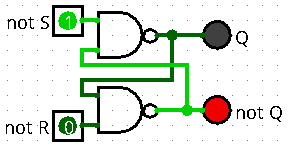
\includegraphics[width=\textwidth]{async-rs-nand}
\end{figure}

\section{Одноступенчатый асинхронный RS-триггер на элементах ИЛИ-НЕ}
Таблица переходов триггера (\cref{tab:async-rs-nor}) и его функциональная схема (\cref{fig:async-rs-nor}).

\begin{table}[H]
	\caption{Таблица переходов асинхронного RS-триггера на элементах ИЛИ-НЕ}
	\label{tab:async-rs-nor}
	\begin{tabular}{|c|c|c|c|c|}
		\hline
		S & R & $Q(t + 1)$ & $\overline{Q(t + 1)}$ & Режим \\
		\hline
		0 & 0 & $Q(t)$ & $\overline{Q(t)}$ & Хранение \\
		\hline
		0 & 1 & 0 & 1 & Установка 0 \\
		\hline
		1 & 0 & 1 & 0 & Установка 1 \\
		\hline
		1 & 1 & 0 & 0 & Запрещенная комбинация \\
		\hline
	\end{tabular}
\end{table}

\begin{figure}[H]
	\caption{Функциональная схема асинхронного RS-триггера на элементах ИЛИ-НЕ}
	\label{fig:async-rs-nor}
	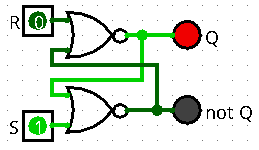
\includegraphics[width=\textwidth]{async-rs-nor}
\end{figure}

\section{Одноступенчатый синхронный RS-триггер на элементах И-НЕ}
Таблица переходов триггера (\cref{tab:sync-rs-nand}) и его функциональная схема (\cref{fig:sync-rs-nand}).

\begin{table}[H]
	\caption{Таблица переходов синхронного RS-триггера на элементах И-НЕ}
	\label{tab:sync-rs-nand}
	\begin{tabular}{|c|c|c|c|c|c|}
		\hline
		C & S & R & $Q(t + 1)$ & $\overline{Q(t + 1)}$ & Режим \\
		\hline
		0 & * & * & $Q(t)$ & $\overline{Q(t)}$ & Хранение \\
		\hline
		1 & 0 & 0 & $Q(t)$ & $\overline{Q(t)}$ & Хранение \\
		\hline
		1 & 0 & 1 & 0 & 1 & Установка 0 \\
		\hline
		1 & 1 & 0 & 1 & 0 & Установка 1 \\
		\hline
		1 & 1 & 1 & 1 & 1 & Запрещенная комбинация \\
		\hline
	\end{tabular}
\end{table}

\begin{figure}[H]
	\caption{Функциональная схема синхронного RS-триггера на элементах И-НЕ}
	\label{fig:sync-rs-nand}
	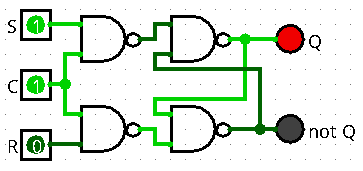
\includegraphics[width=\textwidth]{sync-rs-nand}
\end{figure}

\section{Двухступенчатый синхронный RS-триггер с асинхронными входами предустановки, выполненный на элементах И-НЕ}
Таблица переходов триггера (\cref{tab:dual-sync-rs-nand}) и его функциональная схема (\cref{fig:dual-sync-rs-nand}).

\begin{table}[H]
	\caption{Таблица переходов двухступенчатого синхронного RS-триггера на элементах И-НЕ}
	\label{tab:dual-sync-rs-nand}
	\begin{tabular}{|c|c|c|c|c|c|c|c|}
		\hline
		C & $\overline{S}$ & $\overline{R}$ & S & R & $Q(t + 1)$ & $\overline{Q(t + 1)}$ & Режим \\
		\hline
		* & 0 & 0 & * & * & 1 & 1 & Запрещенная комбинация \\
		\hline
		* & 0 & 1 & * & * & 1 & 0 & Асинхронная 1 \\
		\hline
		* & 1 & 0 & * & * & 0 & 1 & Асинхронный 0 \\
		\hline
		0 & 1 & 1 & * & * & $Q(t)$ & $\overline{Q(t)}$ & Хранение \\
		\hline
		1 & 1 & 1 & * & * & $Q(t)$ & $\overline{Q(t)}$ & Хранение \\
		\hline
		\clockbt & 1 & 1 & 0 & 1 & 0 & 1 & Синхронная установка 0 \\
		\hline
		\clockbt & 1 & 1 & 1 & 0 & 1 & 0 & Синхронная установка 1 \\
		\hline
		\clockbt & 1 & 1 & 1 & 1 & 1 & 1 & Запрещенная комбинация \\
		\hline
	\end{tabular}
\end{table}

\begin{figure}[H]
	\caption{Функциональная схема двухступенчатого синхронного RS-триггера на элементах И-НЕ}
	\label{fig:dual-sync-rs-nand}
	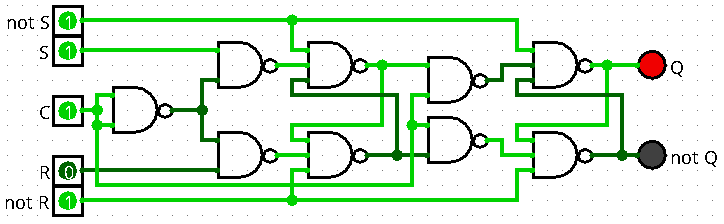
\includegraphics[width=\textwidth]{dual-sync-rs-nand}
\end{figure}

\section{Одноступенчатый D-триггер, выполненный на элементах И-НЕ}
Таблица переходов триггера (\cref{tab:d-nand}) и его функциональная схема (\cref{fig:d-nand}).

\begin{table}[H]
	\caption{Таблица переходов одноступенчатого D-триггера на элементах И-НЕ}
	\label{tab:d-nand}
	\begin{tabular}{|c|c|c|c|c|}
		\hline
		C & D & $Q(t + 1)$ & $\overline{Q(t + 1)}$ & Режим \\
		\hline
		0 & * & $Q(t)$ & $\overline{Q(t)}$ & Хранение \\
		\hline
		1 & 0 & 0 & 1 & Установка 0 \\
		\hline
		1 & 1 & 1 & 0 & Установка 1 \\
		\hline
	\end{tabular}
\end{table}

\begin{figure}[H]
	\caption{Функциональная схема одноступенчатого D-триггера на элементах И-НЕ}
	\label{fig:d-nand}
	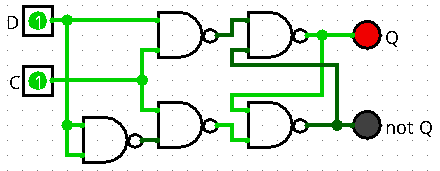
\includegraphics[width=\textwidth]{d-nand}
\end{figure}

\section{Динамический RS-триггер, работающий по переднему фронту, выполненный на элементах И-НЕ}
Таблица переходов триггера (\cref{tab:dynamic-rs-nand}) и его функциональная схема (\cref{fig:dynamic-rs-nand}).

\begin{table}[H]
	\caption{Таблица переходов динамического RS-триггера на элементах И-НЕ}
	\label{tab:dynamic-rs-nand}
	\begin{tabular}{|c|c|c|c|c|c|}
		\hline
		C & $\overline{S}$ & $\overline{R}$ & $Q(t + 1)$ & $\overline{Q(t + 1)}$ & Режим \\
		\hline
		0 & * & * & $Q(t)$ & $\overline{Q(t)}$ & Хранение \\
		\hline
		1 & * & * & $Q(t)$ & $\overline{Q(t)}$ & Хранение \\
		\hline
		\clockbt & 0 & 0 & 0 & 0 & Запрещенная комбинация \\
		\hline
		\clockbt & 0 & 1 & 1 & 0 & Синхронная установка 1 \\
		\hline
		\clockbt & 1 & 0 & 0 & 1 & Синхронная установка 0 \\
		\hline
		* & 1 & 1 & $Q(t)$ & $\overline{Q(t)}$ & Хранение \\
		\hline
	\end{tabular}
\end{table}

\begin{figure}[H]
	\caption{Функциональная схема динамического RS-триггера на элементах И-НЕ}
	\label{fig:dynamic-rs-nand}
	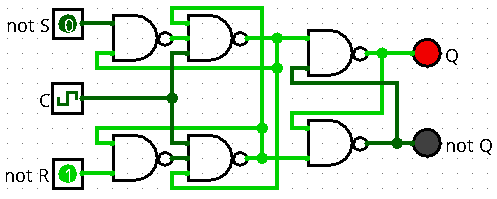
\includegraphics[width=\textwidth]{dynamic-rs-nand}
\end{figure}

\section{Динамический RS-триггер, работающий по заднему фронту, выполненный на элементах ИЛИ-НЕ}
Таблица переходов триггера (\cref{tab:dynamic-rs-nor}) и его функциональная схема (\cref{fig:dynamic-rs-nor}).

\begin{table}[H]
	\caption{Таблица переходов динамического RS-триггера на элементах ИЛИ-НЕ}
	\label{tab:dynamic-rs-nor}
	\begin{tabular}{|c|c|c|c|c|c|}
		\hline
		C & $\overline{S}$ & $\overline{R}$ & $Q(t + 1)$ & $\overline{Q(t + 1)}$ & Режим \\
		\hline
		0 & * & * & $Q(t)$ & $\overline{Q(t)}$ & Хранение \\
		\hline
		1 & * & * & $Q(t)$ & $\overline{Q(t)}$ & Хранение \\
		\hline
		\clocktb & 1 & 1 & 1 & 1 & Запрещенная комбинация \\
		\hline
		\clocktb & 0 & 1 & 1 & 0 & Синхронная установка 1 \\
		\hline
		\clocktb & 1 & 0 & 0 & 1 & Синхронная установка 0 \\
		\hline
		* & 0 & 0 & $Q(t)$ & $\overline{Q(t)}$ & Хранение \\
		\hline
	\end{tabular}
\end{table}

\begin{figure}[H]
	\caption{Функциональная схема динамического RS-триггера на элементах ИЛИ-НЕ}
	\label{fig:dynamic-rs-nor}
	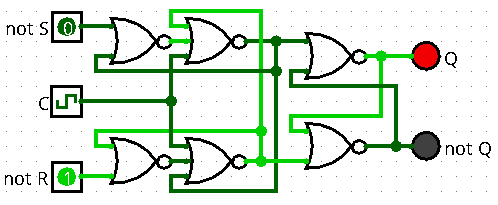
\includegraphics[width=\textwidth]{dynamic-rs-nor}
\end{figure}

\section{Т-триггер с асинхронными входами предустановки, выполненный на основе двухступенчатого RS-триггера}
Таблица переходов триггера (\cref{tab:t-on-dual-rs}) и его функциональная схема (\cref{fig:t-on-dual-rs}).

\begin{table}[H]
	\caption{Таблица переходов T-триггера}
	\label{tab:t-on-dual-rs}
	\begin{tabular}{|c|c|c|c|c|c|}
		\hline
		T & $\overline{S}$ & $\overline{R}$ & $Q(t + 1)$ & $\overline{Q(t + 1)}$ & Режим \\
		\hline
		* & 0 & 0 & 1 & 1 & Запрещенная комбинация \\
		\hline
		* & 0 & 1 & 1 & 0 & Асинхронная 1 \\
		\hline
		* & 1 & 0 & 0 & 1 & Асинхронный 0 \\
		\hline
		0 & 1 & 1 & $Q(t)$ & $\overline{Q(t)}$ & Хранение \\
		\hline
		1 & 1 & 1 & $Q(t)$ & $\overline{Q(t)}$ & Хранение \\
		\hline
		\clockbt & 1 & 1 & $\overline{Q(t)}$ & $Q(t)$ & Переключение в противоположное состояние \\
		\hline
	\end{tabular}
\end{table}

\begin{figure}[H]
	\caption{Функциональная схема T-триггера}
	\label{fig:t-on-dual-rs}
	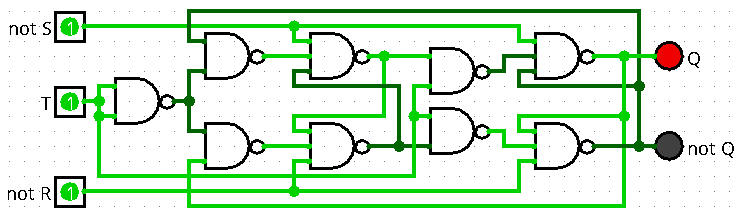
\includegraphics[width=\textwidth]{t-on-dual-rs}
\end{figure}

\section{JK-триггер}
Таблица переходов триггера (\cref{tab:jk}) и его функциональная схема (\cref{fig:jk}).

\begin{table}[H]
	\caption{Таблица переходов JK-триггера}
	\label{tab:jk}
	\begin{tabular}{|c|c|c|c|c|c|c|c|}
		\hline
		C & $\overline{S}$ & $\overline{R}$ & J & K & $Q(t + 1)$ & $\overline{Q(t + 1)}$ & Режим \\
		\hline
		* & 0 & 0 & * & * & 1 & 1 & Запрещенная комбинация \\
		\hline
		* & 0 & 1 & * & * & 1 & 0 & Асинхронная 1 \\
		\hline
		* & 1 & 0 & * & * & 0 & 1 & Асинхронный 0 \\
		\hline
		0 & 1 & 1 & * & * & $Q(t)$ & $\overline{Q(t)}$ & Хранение \\
		\hline
		1 & 1 & 1 & 1 & \clocktb & 0 & 1 & Подмена входов C и K \\
		\hline
		1 & 1 & 1 & \clocktb & 1 & 1 & 1 & Подмена входов C и R \\
		\hline
		1 & 1 & 1 & \clocktb & 1 & 1 & 1 & Подмена входов C и R \\
		\hline
		\clocktb & 1 & 1 & 0 & 1 & 0 & 1 & Синхронная установка 0 \\
		\hline
		\clocktb & 1 & 1 & 1 & 0 & 1 & 0 & Синхронная установка 1 \\
		\hline
		\clocktb & 1 & 1 & 1 & 1 & 1 & 1 & Режим T-триггера \\
		\hline
	\end{tabular}
\end{table}

\begin{figure}[H]
	\caption{Функциональная схема JK-триггера}
	\label{fig:jk}
	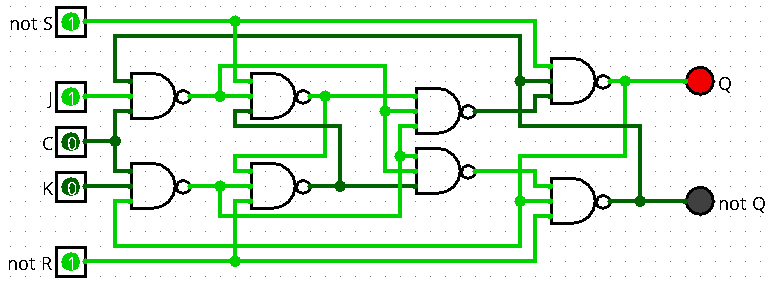
\includegraphics[width=\textwidth]{jk}
\end{figure}

\chapter{Выводы}
В ходе работы на практике была изучена работа триггеров.

\chapter{Информационный источник}
\textbf{Смирнов, С. С.} Информатика : Методические указания по выполнению практических работ / С. С. Смирнов, Д. А. Карпов. -- Москва : МИРЭА -- Российский технологический университет, 2020. -- 102 с.

\end{document}
